\documentclass[11pt]{article}
\usepackage[a4paper,margin=2.4cm]{geometry}
\usepackage{booktabs}
\usepackage{graphicx}
\usepackage{amsmath}
\usepackage{xcolor}
\usepackage{hyperref}
\hypersetup{colorlinks=true,linkcolor=blue,urlcolor=blue}
\usepackage{caption}
\captionsetup{font=small}
\setlength{\parskip}{0.4em}
\setlength{\parindent}{0pt}

\title{\textbf{Pocket-Overlap Audit of RankBind's Residue Attention}\\[2pt]
\large Does Stage-(b) attention attend to catalytic / binding residues?}
\author{RankBind supplementary analysis}
\date{2026-06-04}

\begin{document}
\maketitle

\section*{Summary}

The residue-level extension of RankBind (\emph{Stage-b}, the \texttt{v5b}
model) replaces the v4 mean-pool over per-residue ESM2 embeddings with a
\emph{learned-query attention pool}. An earlier audit established two facts:
the attention weights are near-uniform in \emph{magnitude} (top-10\% of
residues hold only $\sim$11.8\% of the mass), yet their \emph{rank order} is
reproducible across random seeds (Spearman $\rho \approx 0.86$). The paper
deferred the obvious follow-up question to future work:
\emph{is that reproducible rank order pointing at the protein's functional
pocket?}

This report answers it. \textbf{No --- and significantly so.} Across 50
proteins with curated UniProt active-site / binding-site annotations, the
attention weight ranks the annotated pocket residues \emph{below} background
(mean ROC-AUC $0.213$ vs.\ chance $0.50$; Wilcoxon $p < 10^{-4}$). The
attention pool systematically \emph{de-weights} the catalytic and
ligand-binding residues. This is a clean negative result that confirms the
\emph{LayerNorm-then-pool} mechanism the paper proposes and hardens the
argument against an attention-seeded atom-level extension.

\section{Method}

\paragraph{Ground truth.} For each protein we query the UniProt REST API for
residue-level feature annotations and take the union of the
\textbf{Active site} (catalytic) and \textbf{Binding site}
(ligand / cofactor contact) positions as the ``pocket'' label. UniProt's
1-based residue position $p$ maps to embedding row $p-1$; we verified that the
stored ESM2 per-residue tensor has exactly one row per UniProt residue (no
\texttt{CLS}/\texttt{EOS} offset) by matching sequence lengths.

\paragraph{Predictor.} For each protein we extract the per-residue attention
weight $\alpha_i \in [0,1]$ (the softmax coefficient that multiplies residue
$i$ in the pooled vector) from each of the three trained seeds
$\{42, 7, 1337\}$, and average them into a cross-seed \emph{consensus} weight
--- the reproducible signal the paper highlights.

\paragraph{Metrics (per protein).} Treating annotated residues as positives
and the attention weight as the score:
\begin{itemize}\setlength\itemsep{0pt}
  \item \textbf{ROC-AUC} --- probability the weight ranks a random pocket
        residue above a random non-pocket residue. $0.5=$ chance; $>0.5=$
        attention concentrates on the pocket; $<0.5=$ attention avoids it.
  \item \textbf{mean percentile} --- average percentile-rank of the pocket
        residues' weights ($0.5=$ chance).
  \item \textbf{enrichment} --- mean weight on pocket residues divided by the
        mean weight over all residues ($1.0=$ no preference).
  \item \textbf{top-10\% enrichment} --- fraction of pocket residues landing
        in the protein's $10\%$ most-attended residues, divided by the chance
        rate $0.10$ ($1.0=$ chance).
\end{itemize}

\section{Results}

\paragraph{The six figure proteins.} These are the panels of
\texttt{fig\_attn\_weight\_examples.png} in the paper. Five of six de-weight the
pocket; only Q77J78 is enriched.

\begin{table}[h]
\centering
\small
\begin{tabular}{lrrrrrr}
\toprule
UniProt & len & \#pocket & ROC-AUC & mean pctile & enrich. & top-10\% enr. \\
\midrule
Q77J78     & 461 & 5 & \textbf{0.729} & 0.727 & 1.051 & 4.00 \\
Q65MI2     & 562 & 5 & 0.396 & 0.397 & 0.960 & 0.00 \\
Q8A6L0     & 662 & 4 & 0.304 & 0.304 & 0.925 & 0.00 \\
P08311     & 255 & 3 & 0.070 & 0.073 & 0.770 & 0.00 \\
O25046     & 409 & 4 & 0.019 & 0.022 & 0.807 & 0.00 \\
A0A1L9P8I4 & 608 & 1 & 0.012 & 0.012 & 0.802 & 0.00 \\
\midrule
\textbf{mean} & & & \textbf{0.255} & 0.256 & 0.886 & 0.67 \\
\bottomrule
\end{tabular}
\caption{Pocket overlap for the six attention-figure proteins
(cross-seed consensus weight). Chance baselines: ROC-AUC $0.50$, mean
percentile $0.50$, enrichment $1.00$, top-10\% enrichment $1.00$.}
\end{table}

\paragraph{Full sample (50 proteins).} The trend is robust and statistically
significant: 43 of 50 proteins fall below the chance AUC of $0.50$.

\begin{table}[h]
\centering
\small
\begin{tabular}{lrrrr}
\toprule
 & ROC-AUC & mean pctile & enrichment & top-10\% enr. \\
\midrule
mean             & \textbf{0.213} & 0.217 & 0.876 & 0.43 \\
median           & 0.129 & --- & --- & --- \\
chance           & 0.500 & 0.500 & 1.000 & 1.00 \\
\# below chance  & 43 / 50 & --- & --- & --- \\
\bottomrule
\end{tabular}
\caption{Cross-seed consensus pocket overlap over all 50 sampled proteins with
UniProt active/binding-site annotations. Wilcoxon signed-rank test of ROC-AUC
against $0.50$: $p < 10^{-4}$.}
\end{table}

\begin{figure}[h]
\centering
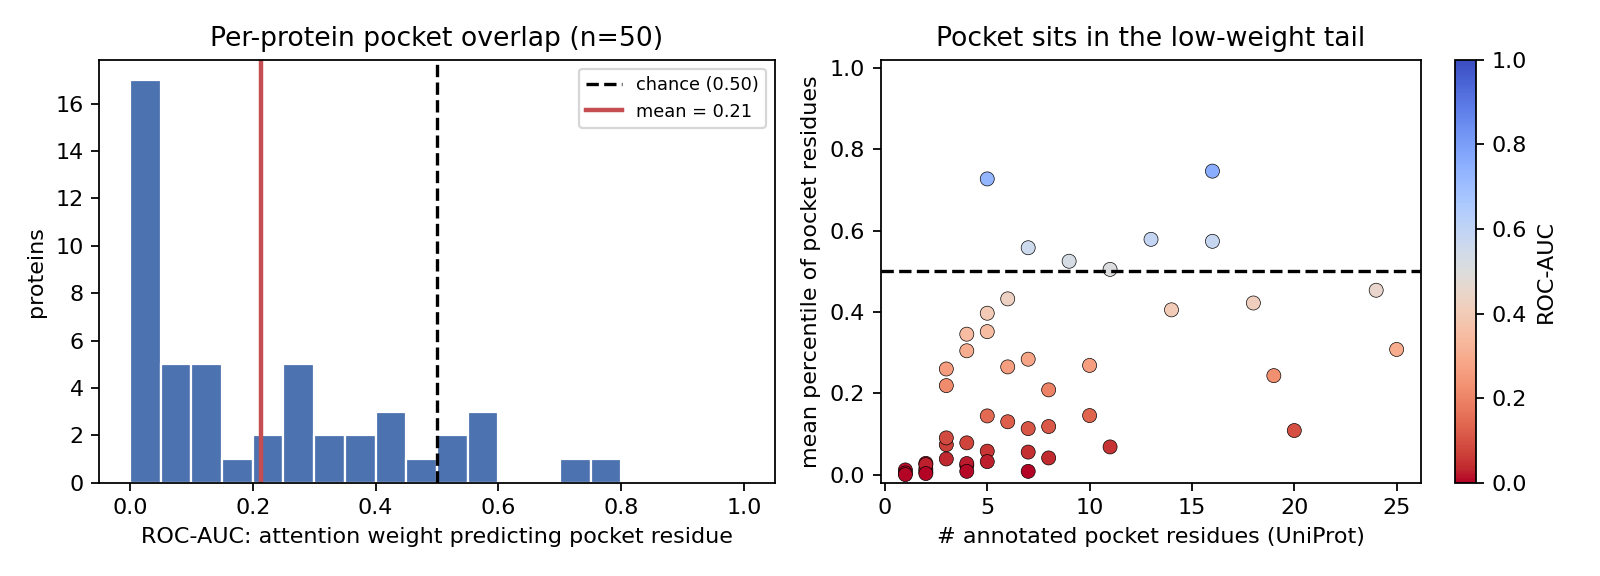
\includegraphics[width=\linewidth]{figures/fig_pocket_overlap.png}
\caption{\textbf{Left:} distribution of per-protein ROC-AUC. The mass sits
well below the chance line at $0.50$; the mean is $0.21$. \textbf{Right:} mean
percentile of the annotated pocket residues against the number of annotated
residues, coloured by ROC-AUC. Almost every protein's pocket sits in the
low-weight tail (well below the $0.50$ chance line), independent of how many
residues are annotated.}
\end{figure}

\begin{figure}[h]
\centering
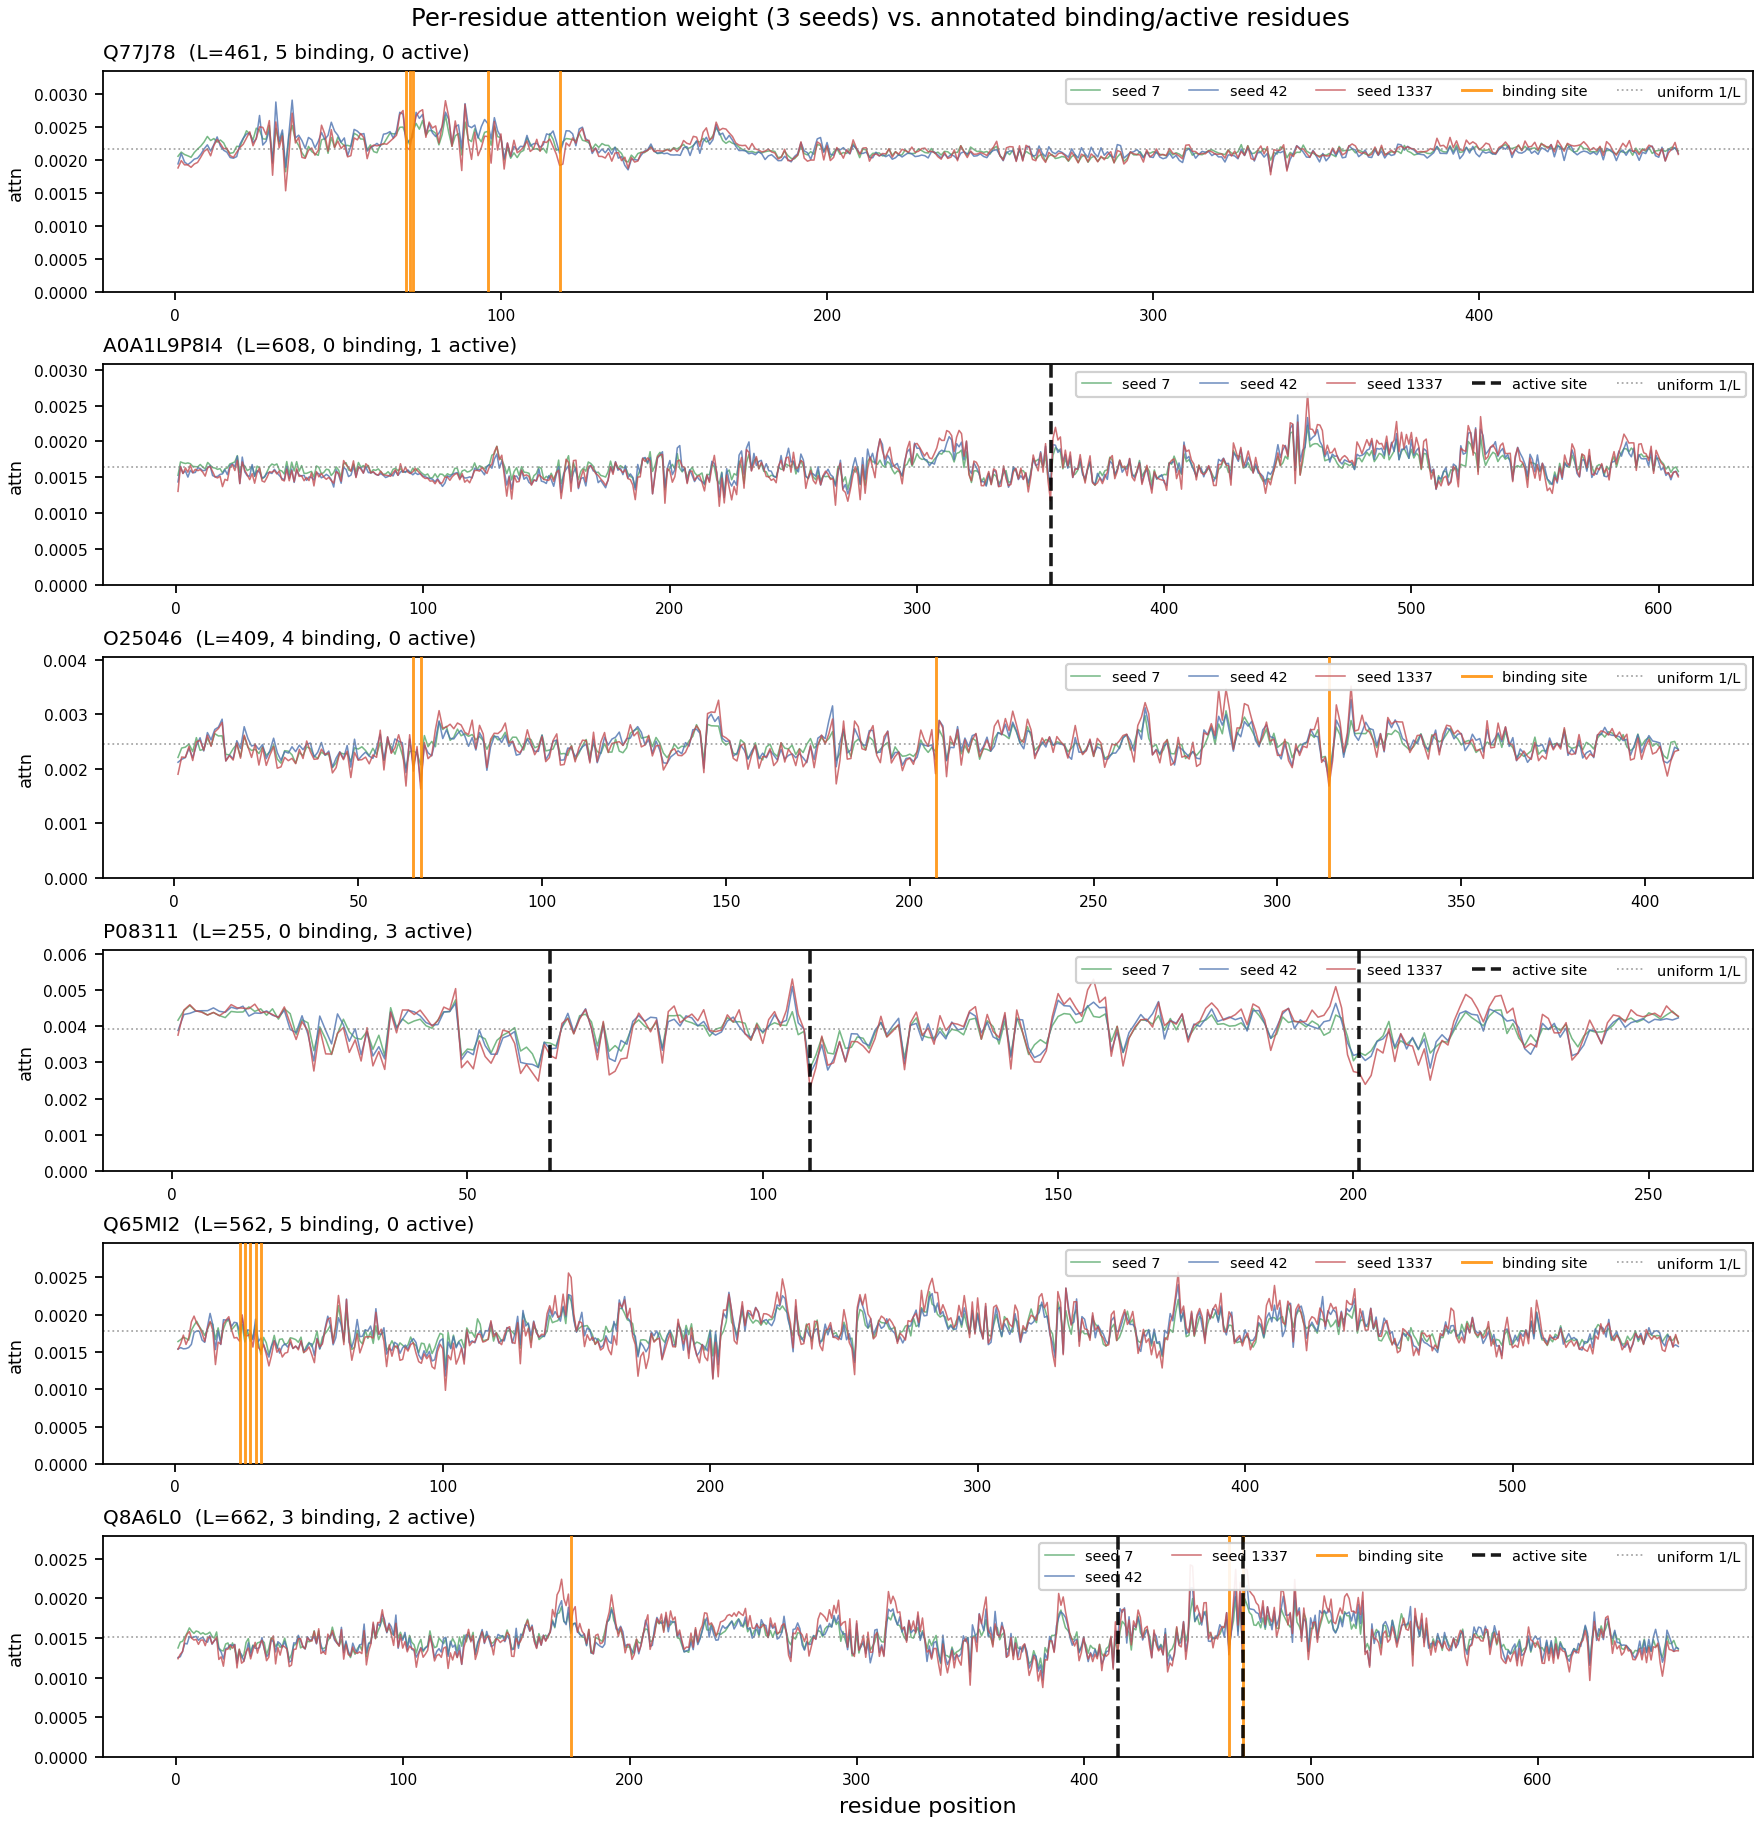
\includegraphics[width=\linewidth]{figures/fig_attn_weight_pocket_examples.png}
\caption{Per-residue attention weight along the sequence for the six
attention-figure proteins, with the three seeds overlaid (blue / green / red).
\textcolor[HTML]{FF8C00}{\textbf{Orange}} verticals mark UniProt
\textbf{binding-site} residues; \textbf{black dashed} verticals mark
\textbf{active-site} residues; the grey dotted line is the uniform weight
$1/L$. The annotated functional residues do not coincide with the attention
peaks --- they typically fall on flat or below-uniform stretches. This is the
visual counterpart of the ROC-AUC $0.21$ result: the curves are jagged and
reproducible across seeds, but their structure is unrelated (if anything,
anti-correlated) to where the protein actually binds.}
\end{figure}

\section{Interpretation}

The attention pool does \emph{not} select the functional pocket; if anything it
reliably points away from it. This is consistent with --- and is direct
evidence for --- the \emph{LayerNorm-then-pool} mechanism the paper proposes
for why Stage-(b) lifts MRR by $+0.10$:

\begin{enumerate}\setlength\itemsep{2pt}
  \item Residues are LayerNorm-normalised \emph{before} the softmax. The
        learned attention's role is to \emph{tame} high-norm residues so they
        do not dominate the pooled average, not to highlight a binding site.
  \item Catalytic and binding residues are among the most evolutionarily
        conserved, distinctive positions in a protein, and are correspondingly
        high-norm / high-salience in ESM2 representation space --- precisely
        the residues the normalisation suppresses. The measured de-weighting
        (enrichment $0.88 < 1$) is the expected signature of this mechanism.
  \item The cross-seed-reproducible rank order ($\rho \approx 0.86$) is
        therefore \emph{not} a reproducible pocket detector; it is a
        reproducible preference for down-weighting structurally salient
        regions (e.g.\ termini, signal peptides, conserved cores).
\end{enumerate}

\paragraph{Consequence for the deferred atom-level extension.} The originally
pre-registered atom-level stage would have built an atom graph on the
top-$K{=}8$ most-attended residues plus their $4$\,\AA{} neighbourhood. This
audit blocks that mechanism a second way: beyond the weights being near-uniform
and only $50\%$ reproducible across seeds at the top-10\%, they are
\emph{anti}-correlated with the pocket --- so the most-attended residues are
the \emph{worst} possible seed set for a pocket graph. A redesigned variant
must derive the pocket from structure (e.g.\ \texttt{fpocket} on AlphaFold
models or EC-class catalytic motifs), not from attention.

\paragraph{Honesty / limitations.} UniProt active/binding-site annotations are
sparse (1--20 residues per protein here) and some are inferred by homology
rather than measured. We mitigate this with $n=50$ proteins and a non-parametric
test; the effect is large and consistent (43/50 below chance, $p<10^{-4}$), so
it is not an artefact of a few mis-annotated proteins. The audit speaks to
attention \emph{magnitude} localisation only; it does not claim the residue
branch carries no structural information --- only that whatever it carries is
not expressed as pocket-localised attention mass.

\section*{Reproducibility}

\begin{tabular}{ll}
Script & \texttt{evaluation/attn\_pocket\_overlap.py} \\
Data (6 figure proteins) & \texttt{evaluation/attractor\_results/attn\_pocket\_overlap.csv} \\
Data (50 proteins) & \texttt{evaluation/attractor\_results/attn\_pocket\_overlap\_all.csv} \\
Figure & \texttt{paper/figures/fig\_pocket\_overlap.png} \\
Models & \texttt{results/v5\_rankbind/*abl\_attn\_pool\_v5b\_s\{42,7,1337\}} \\
Command & \texttt{python -m evaluation.attn\_pocket\_overlap [--all]} \\
\end{tabular}

\end{document}
